\chapter{Depth data acquisition techniques}
\label{cha:acquisition}

\begin{comment}
[1] - Build Your Own 3D Scanner

What is a depth map. Classification of aqcuisition methods - passive and active, number of vantage points. This chapter provides a brief description of the operating principle of some commonly used techniques with their advantages and disadvantages.
\end{comment}


The manipulation and movement tasks of a MMS robot involves continuous interaction with unstructured and changing environment. In order to develop an autonomous system, which will be able to operate in such conditions, a data acquisition system is required, that would provide the necessary information about the nearby objects surface, size and relative distances. The measurement of this type can be performed by using depth acquisition techniques, also known as three dimensional (3D) imaging.

The first depth acquisition techniques emerged as a replacement for a contact-based coordinate measuring machines (CMM). CMMs were used in the industrial quality control applications and worked by recording the displacement of a probe tip sliding across a solid surface. Such method was time consuming and inadequate for fragile objects. Modern, contact-less 3D scanning apparatus overcome those limitations by using light to interact with the environment. The new technology has also extended the application area of 3D scanning to the field of robotic perception.

Modern methods of 3D data acquisition are classified by the light source they utilize to measure depth. \textit{Passive} techniques rely only on the ambient light, whereas the \textit{active} ones operate by projecting illumination onto an object and recording the reflected beam. In the following sections, examples of both categories are presented, with a brief description of their principles of operation and a discussion of advantages and disadvantages, finalized by hardware selection for the designed MMS robot.

%-------------------------------------------------------

\section{Stereo vision}
\label{sec:stereo}

\begin{comment}
[1] - State-Of-The-Art and Applications of 3D imaging sensors
Pic: http://zone.ni.com/reference/en-XX/help/372916M-01/nivisionconceptsdita/guid-cb42607e-f256-40f5-ab6e-28ec3a33bcda/

Passive method. Based on human vision - biological process of Stereopsis. Depth info acquired using two or more images concurrently captured from displaced cameras. Processing steps: image acquisition, camera modeling, feature extractions, correspondence analysis and triangulation. Simple, low-cost hardware, but processing computationally expensive. Features? Correspondences? Triangulation with picture.

\end{comment}

Stereo vision is a passive depth acquisition technique, widely used in research and  industry. Its principle of operation is based on human vision system and the biological process of stereopsis, where the disparity between two different projections of the world on the human retinas leads to the depth sensation. Analogically, in computer stereo vision technique, two (or more) displaced in space cameras concurrently acquire the scene view. From the captured images disparity, a scene depth information is then inferred. A typical scheme for stereo vision depth calculation after image acquisition is divided into two steps: the correspondence problem and triangulation.

The correspondence problem is the most difficult part of the stereo vision. It can be stated as follows: given two displaced 2D images of the same scene, find points representing the same space location in those images. There are many point matching algorithms discussed in the literature. Some of them rely on computing point features, based on their neighbourhood, while others compute statistical descriptors of characteristic areas in the image, and then minimise the measured difference between analysed regions to find the best matches. The correspondence problem in computer vision is a wide and open research area, that is beyond the scope of this work. A thorough description of the problem and its solutions, is provided, for example, by \cite{Cyganek}.

\begin{figure}[H]
\label{fig:stereo}
\centering
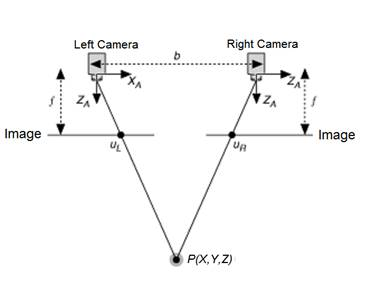
\includegraphics[width=0.5\textwidth]{fig/nistereovision}
\caption{A simplified stereo vision system \cite{nistereo}}
\label{fig:stereovision}
\end{figure}


After obtaining the corresponding points, the point depth information can be derived by the means of triangulation (Figure \ref{fig:stereovision}). if the imaging properties of the camera are known, two three-dimensional lines, from the camera's projection centres to the examined point can be drawn. The intersection of those lines is then used to infer the depth of the point. 

The main advantage of the stereo vision system is that it can be built with easily accessible, standard 2D cameras. Such cameras allow to reduce the expenditure and provide relatively high resolution. On the other hand, the stereo vision systems have many drawbacks. Firstly, their performance is reduced in environments with low ambient light intensity, which makes the system impractical in some settings. Secondly, the depth accuracy decreases quadratically with the distance. Finally, the algorithms used for feature extraction and matching, involved in solving the correspondence problem are computationally expensive and often limit the depth acquisition frame rate.


 There also exists a variant of active stereo vision, utilized i.e. in the Ensenso N10 cameras \cite{ensenso}. In this case, besides the camera pair, a pattern projector is applied to add artificial texture to the scene, which helps to determine the disparity on untextured surfaces.



\begin{comment}
WIKIPEDIA:

Computer stereo vision is the extraction of 3D information from digital images, such as obtained by a CCD camera. By comparing information about a scene from two vantage points, 3D information can be extracted by examination of the relative positions of objects in the two panels. This is similar to the biological process Stereopsis.

\begin{figure}[H]
\centering
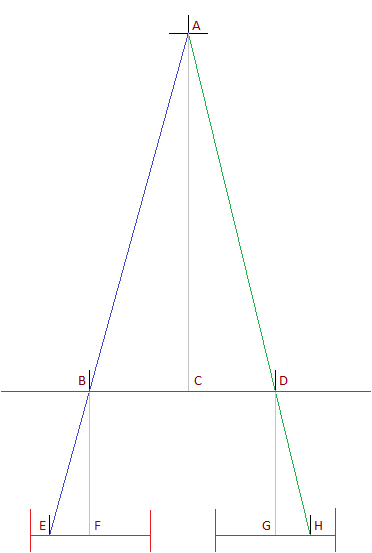
\includegraphics[scale=0.7]{stereo}
\caption{Stereo vision}
\end{figure}

In traditional stereo vision, two cameras, displaced horizontally from one another are used to obtain two differing views on a scene, in a manner similar to human binocular vision. By comparing these two images, the relative depth information can be obtained, in the form of disparities, which are inversely proportional to the differences in distance to the objects.

To compare the images, the two views must be superimposed in a stereoscopic device, the image from the right camera being shown to the observer's right eye and from the left one to the left eye.

In real camera systems however, several pre-processing steps are required.

The image must first be removed of distortions, such as barrel distortion to ensure that the observed image is purely projectional.
The image must be projected back to a common plane to allow comparison of the image pairs, known as image rectification.
An information measure which compares the two images is minimized. This gives the best estimate of the position of features in the two images, and creates a disparity map.
Optionally, the disparity as observed by the common projection, is converted back to the height map by inversion. Utilising the correct proportionality constant, the height map can be calibrated to provide exact distances.
%---------------------------------------------------------------------------
\end{comment}


\begin{comment}
%\section{Laser LIDAR}
%\label{sec:lidar}

WIKIPEDIA:


Lidar (also written LIDAR or LiDAR) is a remote sensing technology that measures distance by illuminating a target with a laser and analyzing the reflected light. Although thought by some to be an acronym of Light Detection And Ranging, the term lidar was actually created as a portmanteau of "light" and "radar."

Lidar is popularly used as a technology to make high-resolution maps, with applications in geomatics, archaeology, geography, geology, geomorphology, seismology, forestry, remote sensing, atmospheric physics, airborne laser swath mapping (ALSM), laser altimetry, and contour mapping.

Lidar uses ultraviolet, visible, or near infrared light to image objects. It can target a wide range of materials, including non-metallic objects, rocks, rain, chemical compounds, aerosols, clouds and even single molecules.[4] A narrow laser-beam can map physical features with very high resolution[vague].

Lidar has been used extensively for atmospheric research and meteorology. Lidar instruments fitted to aircraft and satellites carry out surveying and mapping – a recent example being the U.S. Geological Survey Experimental Advanced Airborne Research Lidar.[12] NASA has identified lidar as a key technology for enabling autonomous precision safe landing of future robotic and crewed lunar-landing vehicles.[13]

Wavelengths vary to suit the target: from about 10 micrometers to the UV (approximately 250 nm). Typically light is reflected via backscattering. Different types of scattering are used for different lidar applications: most commonly Rayleigh scattering, Mie scattering, Raman scattering, and fluorescence. Based on different kinds of backscattering, the lidar can be accordingly called Rayleigh Lidar, Mie Lidar, Raman Lidar, Na/Fe/K Fluorescence Lidar, and so on.[4] Suitable combinations of wavelengths can allow for remote mapping of atmospheric contents by identifying wavelength-dependent changes in the intensity of the returned signal.

\end{comment}
%---------------------------------------------------------------------------

\section{Time of flight}
\label{sec:tof}

\begin{comment}
http://www.ti.com/lit/wp/sloa190b/sloa190b.pdf
\end{comment}

Time of flight (ToF) cameras work on a completely different principle than stereoscopic systems. ToF systems are characterised with active illumination and are composed of an near infra-red (IR) emmiter and IR camera. They work by illuminating the scene with a modulated IR beam and recording the received light, as presented in the figure 5. The distance from the recorded object is then calculated by measuring the phase shift between the illuminated and reflected signals. 

In the simplest form, the ToF cameras use single light pulses \cite{titof}. After a short period of illumination, the reflected energy is then integrated at every pixel with two out of phase windows over the same $\Delta t$ time, resulting in two electrical charges $Q_1$ and $Q_2$. The depth distance $d$ is then computed as $d = \frac{1}{2}c\Delta t \frac{Q_2}{Q_1+Q_2}$, where $c$ is the speed of light constant. A more advanced method is to project illumination modulated by a continuous wave signal, commonly a square wave. In this case, four sampling windows, shifted by \SI{90}{\degree} angle, resulting in $Q_1$,$Q_2$, $Q_3$ and $Q_4$ charges. The phase angle $\phi$ between the projected and the reflected signals is given by $\phi = arctan \frac{Q_3 - Q_4}{Q_1 - Q_2} $ and the final depth $d = \frac{c}{4\pi f}\phi$. The principle of the continuous wave method is illustrated by the Figure \ref{fig:tofprinciple}.

ToF cameras, due to their specific architecture, are prone to errors caused by radiometric, geometric and illumination variations. The power of the emitted IR signal limits their measurement accuracy. The light entering to the sensor has an ambient and reflected components, thus high ambient light intensity reduces the signal to noise ratio. Moreover, the material and color of the object surface cause variations in the amplitude of the reflected IR signal.

\begin{figure}[H]
\label{fig:tof}
\centering
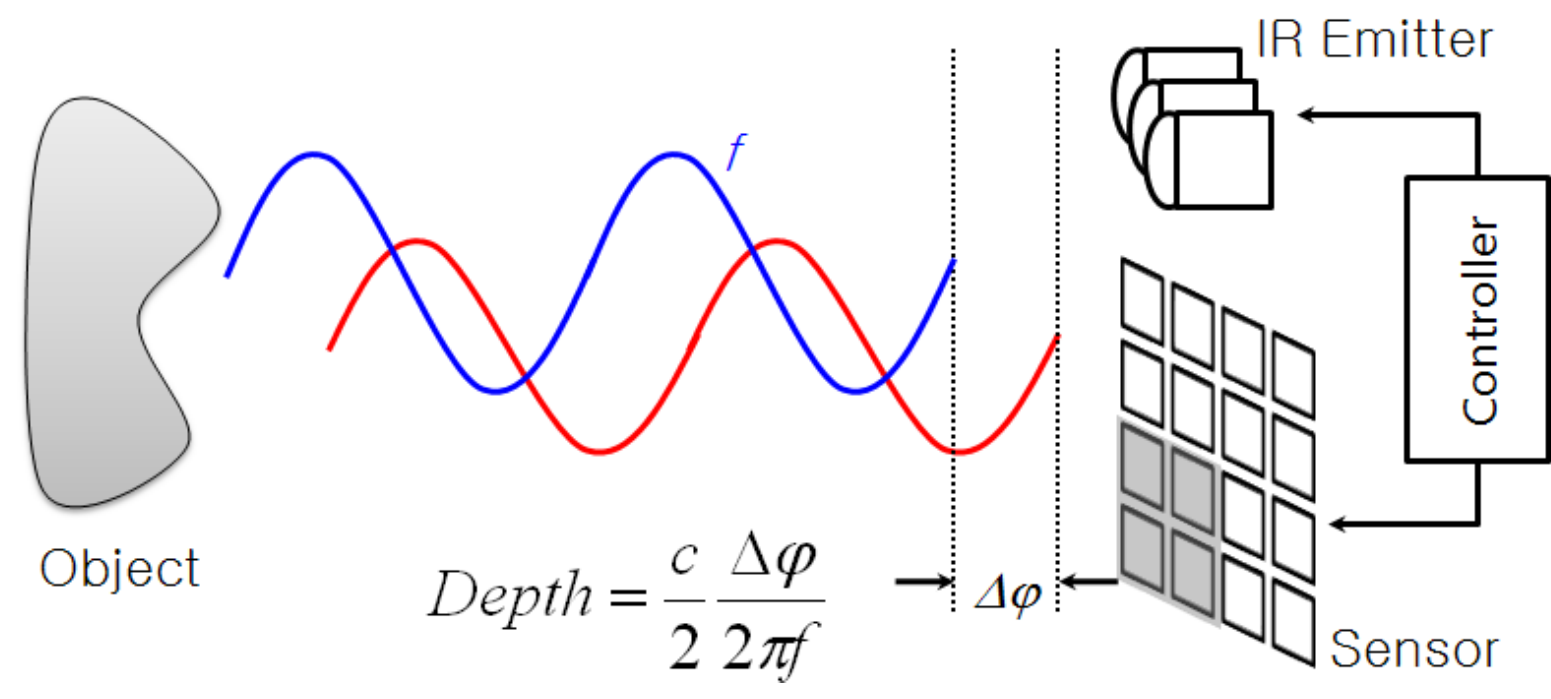
\includegraphics[width=0.7\textwidth]{fig/tofprinciple}
\caption{Time of flight with continuous wave modulation \cite{ToFbook}}
\label{fig:tofprinciple}
\end{figure}

Despite problems arising from ToF principle of operation, modern ToF cameras are distinguished by relatively low latency and fast scanning speed. The depth measurements are acquired directly from the hardware, so the speed is not limited by software processing. Unfortunately, most of the products available on the end-user market provide relatively low depth image resolution, typically QQVGA (160x120) and the price increases significantly with the resolution.


\begin{comment}
WIKIPEDIA:


A time-of-flight camera (ToF camera) is a range imaging camera system that resolves distance based on the known speed of light, measuring the time-of-flight of a light signal between the camera and the subject for each point of the image. The time-of-flight camera is a class of scannerless LIDAR, in which the entire scene is captured with each laser or light pulse, as opposed to point-by-point with a laser beam such as in scanning LIDAR systems.[1]

The simplest version of a time-of-flight camera uses light pulses or a single light pulse. The illumination is switched on for a very short time, the resulting light pulse illuminates the scene and is reflected by the objects in the field of view. The camera lens gathers the reflected light and images it onto the sensor or focal plane array. Depending upon the distance, the incoming light experiences a delay. As light has a speed of approximately c = 300,000,000 meters per second, this delay is very short: an object 2.5 m away will delay the light by 16 ns.

The single pixel consists of a photo sensitive element (e.g. a photo diode). It converts the incoming light into a current. In analog timing imagers, connected to the photo diode are fast switches, which direct the current to one of two (or several) memory elements (e.g. a capacitor) that act as summation elements. In digital timing imagers, a time counter, that can be running at several gigahertz, is connected to each photodetector pixel and stops counting when light is sensed.

Advantages:

Simplicity
In contrast to stereo vision or triangulation systems, the whole system is very compact: the illumination is placed just next to the lens, whereas the other systems need a certain minimum base line. In contrast to laser scanning systems, no mechanical moving parts are needed.

Efficient distance algorithm
It is a direct process to extract the distance information out of the output signals of the TOF sensor. As a result, this task uses only a small amount of processing power, again in contrast to stereo vision, where complex correlation algorithms are implemented. After the distance data has been extracted, object detection, for example, is also a straightforward process to carry out because the algorithms are not disturbed by patterns on the object.

Speed
Time-of-flight cameras are able to measure the distances within a complete scene with a singleshot. As the cameras reach up to 160 frames per second, they are ideally suited to be used in real-time applications.

Disadvantages:

Background light
When using CMOS or other integrating detectors or sensors that use visible or near visible light (400 nm - 700 nm), although most of the background light coming from artificial lighting or the sun is suppressed, the pixel still has to provide a high dynamic range. The background light also generates electrons, which have to be stored. For example, the illumination units in many of today's TOF cameras can provide an illumination level of about 1 watt. The Sun has an illumination power of about 50 watts per square meter after the optical band-pass filter. Therefore, if the illuminated scene has a size of 1 square meter, the light from the sun is 50 times stronger than the modulated signal. For non-integrating TOF sensors that do not integrate light over time and are using near-infrared detectors (InGaAs) to capture the short laser pulse, direct viewing of the sun is a non-issue because the image is not integrated over time, rather captured within a short acquisition cycle typically less than 1 microsecond. Such TOF sensors are used in space applications[19] and in consideration for automotive applications.[24]

Interference
In certain types of TOF devices, if several time-of-flight cameras are running at the same time, the TOF cameras may disturb each other's measurements. To be clear, this is not true of all TOF sensors. There exist several possibilities for dealing with this problem:

Time multiplexing: A control system starts the measurement of the individual cameras consecutively, so that only one illumination unit is active at a time.
Different modulation frequencies: If the cameras modulate their light with different modulation frequencies, their light is collected in the other systems only as background illumination but does not disturb the distance measurement.
For Direct TOF type cameras that use a single laser pulse for illumination, because the single laser pulse is short (e.g. 10 nano-seconds), the round trip TOF to and from the objects in the field of view is correspondingly short (e.g. 100 meters = 660nS TOF round trip), for an imager capturing at 30 Hz, the probability of an interfering interaction is the time that the camera acquisition gate is open divided by the time between laser pulses or approximately 1 in 50,000 (0.66uS divided by 33mS).

Multiple reflections
In contrast to laser scanning systems where a single point is illuminated, the time-of-flight cameras illuminate a whole scene. For a phase difference device (amplitude modulated array), due to multiple reflections, the light may reach the objects along several paths. Therefore, the measured distance may be greater than the true distance. Direct TOF imagers are vulnerable if the light is reflecting from a specular surface. There are published papers available that outline the strengths and weaknesses of the various TOF devices and approaches.

\end{comment}

%---------------------------------------------------------------------------

\section{Structured light}
\label{sec:actuators}

The structured light (SL) depth measurement technique combines some of the features of both time of flight and stereo vision principles.  Similarly to ToF cameras, SL relies on active illumination, work in the near infra-red and is composed of an IR emitter and IR camera. As in the case of stereo vision, depth information is inferred from the disparity between two images by the means of triangulation. In this case, the projected IR pattern is compared with the image captured by the IR camera. The IR projector emits patterns of non-coherent light, which then appears distorted from the perspective of the camera. In such settings, the projection of defined patterns makes explicit correspondences on the reflected image. A typical setting of the SL system is presented in figure 5.


%http://www.extremetech.com/extreme/131159-leap-motion-will-it-make-you-a-magician-or-is-it-just-handwaving
\begin{figure}[H]
\label{fig:sl}
\centering
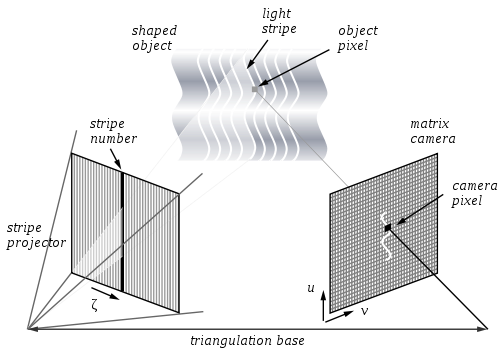
\includegraphics[width=0.6\textwidth]{fig/structuredlight}
\caption{Structured light fringe patterns \cite{extremetech}}
\label{fig:slprinciple}
\end{figure}

	There are many pattern strategies that allow for correspondence identification, including projections of grids, dots, vertical slits and multi-color patterns. In the literature, particular attention is paid to fringe patterns (Figure \ref{fig:slprinciple}), which are suitable to maximize the measurement resolution \cite{sensors}. Moreover, to reduce the reconstruction artifacts, the measurement process is often extended into a sequence of different pattern projections. A comprehensive assessment of such pattern codes can be found in \cite{slcodes}.
	
	Depth measuring devices that employ the SL technique suffer from many drawbacks. Utilizing multiple pattern frames introduces high latency and makes the measurement ill conditioned for dynamic scenes. Moreover, the system performance is degraded in bright ambient light. On the other hand, popular SL devices are characterized with relatively high, VGA (640x480) depth map resolution and are easily accessible on the consumer market.


	A particularly noteworthy application of SL based depth data acquisition device is the Kinect by Microsoft. In addition to an RGB camera and an array of microphones, the device includes an IR projector-camera pair from the PrimeSense Ltd. company, used for depth measurements. The SL light pattern used in Kinect is a non-periodic speckle pattern produced by the interference of partially coherent beams (Figure X). In this device, every pixel is identified in the IR image using a correlation window, after which the depth information is calculated, using triangulation. The Kinect device is produced as a gaming controller for the Xbox 360 console and it is widely available at the consumer market with a relatively low price. Moreover, there are many open source drivers for the Kinect device, which make it a perfect match for robotic and research applications.
	
\begin{figure}[H]
\centering
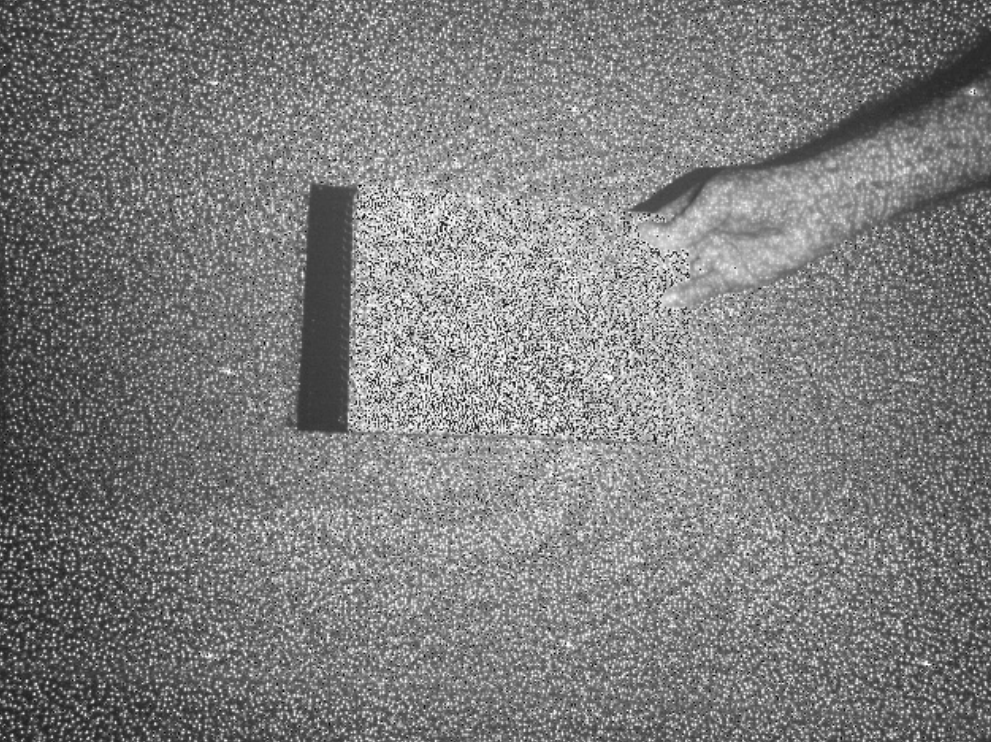
\includegraphics[scale=0.25]{fig/KinectSpeckle}
\caption{Kinect speckle pattern \cite{borenstein2012making}}
\label{fig:kinectspeckle}
\end{figure}
	


\begin{comment}

WIKIPEDIA:


Projecting a narrow band of light onto a three-dimensionally shaped surface produces a line of illumination that appears distorted from other perspectives than that of the projector, and can be used for an exact geometric reconstruction of the surface shape (light section).

A faster and more versatile method is the projection of patterns consisting of many stripes at once, or of arbitrary fringes, as this allows for the acquisition of a multitude of samples simultaneously. Seen from different viewpoints, the pattern appears geometrically distorted due to the surface shape of the object.

Although many other variants of structured light projection are possible, patterns of parallel stripes are widely used. The picture shows the geometrical deformation of a single stripe projected onto a simple 3D surface. The displacement of the stripes allows for an exact retrieval of the 3D coordinates of any details on the object's surface.



Two major methods of stripe pattern generation have been established: Laser interference and projection.

The laser interference method works with two wide planar laser beam fronts. Their interference results in regular, equidistant line patterns. Different pattern sizes can be obtained by changing the angle between these beams. The method allows for the exact and easy generation of very fine patterns with unlimited depth of field. Disadvantages are high cost of implementation, difficulties providing the ideal beam geometry, and laser typical effects like speckle noise and the possible self interference with beam parts reflected from objects. Typically, there is no means of modulating individual stripes, such as with Gray codes.

The projection method uses non coherent light and basically works like a video projector. Patterns are generated by a display within the projector, typically a liquid crystal display (LCD) or liquid crystal on silicon (LCOS) display.

A proprietary projection method uses digital light processing (DLP; moving micro mirror) displays. DLP displays do not absorb light significantly and therefore allow very high light intensities. They also have an extremely linear gray value reproduction, as they are steered by pulse length modulation.

Principally, stripes generated by display projectors have small discontinuities due to the pixel boundaries in the displays. Sufficiently small boundaries however can practically be neglected as they are evened out by the slightest defocus.

A typical measuring assembly consists of one stripe projector and at least one camera. For many applications, two cameras on opposite sides of the projector have been established as useful.

Invisible (or imperceptible) structured light uses structured light without interfering with other computer vision tasks for which the projected pattern will be confusing. Example methods include the use of infrared light or of extremely high framerates alternating between two exact opposite patterns.[2]

There are several depth cues contained in the observed stripe patterns. The displacement of any single stripe can directly be converted into 3D coordinates. For this purpose, the individual stripe has to be identified, which can for example be accomplished by tracing or counting stripes (pattern recognition method). Another common method projects alternating stripe patterns, resulting in binary Gray code sequences identifying the number of each individual stripe hitting the object. An important depth cue also results from the varying stripe widths along the object surface. Stripe width is a function of the steepness of a surface part, i.e. the first derivative of the elevation. Stripe frequency and phase deliver similar cues and can be analyzed by a Fourier transform. Finally, the wavelet transform has recently been discussed for the same purpose.

In many practical implementations, series of measurements combining pattern recognition, Gray codes and Fourier transform are obtained for a complete and unambiguous reconstruction of shapes.

Another method also belonging to the area of fringe projection has been demonstrated, utilizing the depth of field of the camera.[3]

It is also possible to use projected patterns primarily as a means of structure insertion into scenes, for an essentially photogrammetric acquisition.


\end{comment}


\section{Summary and hardware selection}
\label{sec:3dsum}

%http://www.ti.com/ww/en/analog/3dtof/index.shtml?DCMP=hpa_contributed_article&HQS=3dtof-ca

Three of the most popular depth map acquisition techniques were presented in this chapter, including stereo vision, time of flight and structured light. Each method has its advantages and disadvantages and they all have already been successfully applied in robotics. A comparative summary of each method characteristics is presented in Table \ref{tab:depthcompar}.

\begin{table}[h]
\begin{center}
\begin{tabular}{@{}rccc@{}}
\toprule
Feature/Technique                                                                                            & Stereo Vision                                                                                                   & Time of Flight                                                                                                       & Structured Light \\ \midrule
\rowcolor[HTML]{EFEFEF} 
\multicolumn{1}{r|}{\cellcolor[HTML]{EFEFEF}\begin{tabular}[c]{@{}r@{}}Depth data\\ generation\end{tabular}} & \multicolumn{1}{c|}{\cellcolor[HTML]{EFEFEF}\begin{tabular}[c]{@{}c@{}}Directly out \\ of chipset\end{tabular}} & \multicolumn{1}{c|}{\cellcolor[HTML]{EFEFEF}\begin{tabular}[c]{@{}c@{}}High software\\ processing\end{tabular}}      & \begin{tabular}[c]{@{}c@{}}Medium software\\ processing\end{tabular}      \\
\multicolumn{1}{r|}{Latency}                                                                                 & \multicolumn{1}{c|}{Medium}                                                                                     & \multicolumn{1}{c|}{Low}                                                                                             & Medium                                                                    \\
\rowcolor[HTML]{EFEFEF} 
\multicolumn{1}{r|}{\cellcolor[HTML]{EFEFEF}\begin{tabular}[c]{@{}r@{}}Low light\\ performance\end{tabular}} & \multicolumn{1}{c|}{\cellcolor[HTML]{EFEFEF}Weak}                                                               & \multicolumn{1}{c|}{\cellcolor[HTML]{EFEFEF}Good}                                                                    & Good                                                                      \\
\multicolumn{1}{r|}{\begin{tabular}[c]{@{}r@{}}Bright light\\ performance\end{tabular}}                      & \multicolumn{1}{c|}{Good}                                                                                       & \multicolumn{1}{c|}{Medium}                                                                                          & Medium                                                                    \\
\rowcolor[HTML]{EFEFEF} 
\multicolumn{1}{r|}{\cellcolor[HTML]{EFEFEF}\begin{tabular}[c]{@{}r@{}}Power\\ consumption\end{tabular}}     & \multicolumn{1}{c|}{\cellcolor[HTML]{EFEFEF}Low}                                                                & \multicolumn{1}{c|}{\cellcolor[HTML]{EFEFEF}\begin{tabular}[c]{@{}c@{}}Medium - scales\\ with distance\end{tabular}} & \begin{tabular}[c]{@{}c@{}}Medium - scales \\ with distance\end{tabular}  \\
\multicolumn{1}{r|}{Resolution}                                                                              & \multicolumn{1}{c|}{Camera dependent}                                                                           & \multicolumn{1}{c|}{QQVGA, QVGA}                                                                                     & VGA, 1080p                                                                \\
\rowcolor[HTML]{EFEFEF} 
\multicolumn{1}{r|}{\cellcolor[HTML]{EFEFEF}Accurracy}                                                       & \multicolumn{1}{c|}{\cellcolor[HTML]{EFEFEF}mm, cm}                                                              & \multicolumn{1}{c|}{\cellcolor[HTML]{EFEFEF}mm, cm}                                                                  & \SI{}{\micro\meter}, cm                                                                    \\
\multicolumn{1}{r|}{Scanning speed}                                                                          & \multicolumn{1}{c|}{\begin{tabular}[c]{@{}c@{}}Medium - limited by\\  software complexity\end{tabular}}         & \multicolumn{1}{c|}{\begin{tabular}[c]{@{}c@{}}Fast - limited by \\ sensor speed\end{tabular}}                       & \begin{tabular}[c]{@{}c@{}}Fast - limited by\\  camera speed\end{tabular} \\ \bottomrule
\end{tabular}
\caption {Qualitative comparison of depth acquisition techniques \cite{titof}}

\label{tab:depthcompar}
% 2 - http://www.ti.com/ww/en/analog/3dtof/index.shtml?DCMP=hpa_contributed_article&HQS=3dtof-ca
\end{center}
\end{table}

In order to fulfil project assumptions, one solution providing depth map measurement had to be chosen. In the stereo vision technology, ready-made devices unfortunately did not fit within the project budget. Utilizing this technique would therefore require an own design of the stereo vision system. Such solution would probably be the least expensive, but require an extensive amount of work and time. Therefore, the author focused on finding a ready-made solution in the remaining technologies. The DepthSense 311 [3] device was found as a representative of the ToF technique, and the Asus Xtion Pro Live [4] was considered as an option from the SL method. Both devices are available in similiar prices and provide the same frame rate of 30 frames per second. The Asus device, however, offers higher depth map resolution (VGA instead of QQVGA) and has better support from the open source community. The Asus Xtion is based on the PrimeSense Ltd. depth sensing hardware, similarly to the popular Kinect device and is even compatible with the same open source drivers. Nonetheless, it was chosen over the Kinect device, because it has smaller size and is powered directly from the USB port (the Kinect requires external power source). Main specifications of the Asus Xtion Pro device are provided in the Table \ref{tab:asus}.

\begin{table}[h]

\begin{center}

\begin{tabular}{r||l}
\hline
Operating range      & Between 0.8m and 3.5m                                                                   \\

\hline
Field of view        & \SI{58}{\degree H}, \SI{45}{\degree V}, \SI{70}{\degree D} \\

\hline
Depth map resolution & \begin{tabular}[c]{@{}l@{}}VGA (640x480) : 30 fps\\ QVGA (320x240): 60 fps\end{tabular} \\

\hline
Interface            & USB2.0/ 3.0                                                                             \\

\hline
Dimensions           &  18 x 3.5 x 5 cm  \\ \hline
\end{tabular}
\caption{Asus Xtion Pro Live specification \cite{ASUS}}
\label{tab:asus}
\end{center}
\end{table}
